\documentclass[12pt]{book}
\usepackage[english]{babel}
\usepackage{tikz}
\usepackage{graphicx}
\usepackage{changepage} % http://ctan.org/pkg/changepage
\usetikzlibrary{decorations.pathmorphing} % noisy shapes
\usetikzlibrary{fit}		% fitting shapes to coordinates
\usetikzlibrary{backgrounds}	% drawing the background after the foreground
\usepackage{amssymb}
\usepackage{amsmath}
\usepackage{color}

\renewcommand{\labelitemi}{$\bullet$}
\newcommand{\rr}{\raggedright}
\newcommand{\tn}{\tabularnewline}

\title{Bayesian Analysis and Other Cool Stuff}		
\author{Hillary Sanders}	

\begin{document}
\maketitle				

\tableofcontents

\chapter{What is Bayesian Statistics}

\section{Bayesian vs. Classical, Frequentist Statistics}
Bayesian Statistics is a system for statistical inference and decision making which is based on expressing all uncertainty in terms of conditional probability statements. For example: in classical, frequentist statistics, a theory has no $\textit{probability}$ of being correct or incorrect - it is either correct or incorrect, we're just unsure about the truth. But in Bayesian statistics, we're allowed to construct probability models over both observations (data), and beliefs (unknown parameters and theories), and so come up with an actual $p(theory|data)$.
\\\\
There are two aspects of Bayesian Statistics that are important to understand. The first is that unknown variables are not treated as they are in classical, frequentist statistics. In frequentist statistics, even if some value $\theta$ is unknown to us, it is assumed that $\theta$ has some true numeric value. Take the proportion of people in America who like Lady Gaga. A frequentist assumes that there is some true percentage of people in America who like Lady Gaga. And he can estimate that percentage by, for example, asking a (hopefully) random sample of Americans if they like Lady Gaga, and from that he can develop a confidence interval. 
\\\\
Say he gets a 95\% confidence interval from 22\% to 25\%. It's not that he believes that there is a 95\% chance that $\theta$ is somewhere inside the interval [.22, .25], rather that there is a 95\% chance that his confidence interval has overlapped with the fixed, real value of $\theta$. 
\\\\
The Bayesian approach is a little different. A Bayesian might develop a similar confidence interval - say it's [.22, .25] again, and say that she is 95\% sure that $\theta$ is equal to some value in [.22, .25].
% or rather, that the distribution of her beliefs over all possibilities of $\theta$ say that there is a 95\% chance that $\theta$ is in [.22, .25].
\\\\
Foul, you say! Er, at least that's what I said. This is all well and good, but there actually \textit{is}  some fixed, true value of $\theta$. We shouldn't place a distribution over $\theta$ - it's fixed (at least at a fixed time $T$)! Just unknown! Right? Well, sort of. Here's the thing: there's an amazing amount of very powerful methods and tools you can utilize \textit{if} you treat unknown variables like a Bayesian does. And instead of thinking that you're placing a probability distribution over $\theta$, which actually is a bit silly (in most circumstances), you can think of the distribution as a  \textit{distribution of your beliefs} about all possible values of $\theta$ - which, handily enough, can be altered by new, incoming data. 
\\\\
Okay, so that's the first important aspect of Bayesian Statistics: treat unknown variables as variables to be pulled from belief distributions that you define based on information, rather than fixed variables you attempt to estimate. The second important aspect of Bayesian Statistics is the handy result that comes from allowing unknown variables to have probability distributions. Basically, it is the ability to infer a new probability distribution over your unknown variable by using new evidence (data), through the use of Bayes Rule.
\\\\
Ever heard of Bayes Rule? Yeah, I did to in my first statistics class (college, sophomore year), and it pretty much annoyed the heck out of me that something so obvious and intuitive could be named after - in all likelihood - an old white guy who probably believed in God. But, it's important to go over it, because the implications of this formula are very powerful, and very important to understand well.
\\
\begin{equation}
p(A|B) = \frac{p(B|A)*p(A)}{p(B)}
\end{equation}
\\
(If this equation makes total sense to you, skip the following paragraph.)
\\\\
  \def\secondcircle{(210:1.25cm) circle (1.75cm)}
  \def\thirdcircle{(330:.75cm) circle (2.5cm)}
  
\begin{center}
    \begin{tikzpicture}
      \begin{scope}[fill opacity=0.7]
    \fill[gray] \thirdcircle;
     \fill[cyan] \secondcircle;
      \end{scope}

      \draw \secondcircle node [text=black,below left] {$Rain (A)$};
      \draw \thirdcircle node [text=black,below right] {$Clouds (B)$};
    \end{tikzpicture}
    \end{center}
    

In English, this says that the probability of event A, given that event $B$ has happened, is the probability of event $B$ happening, given A, multiplied by the probability of $A$ in the first place (in other words, the probability of both $A$ and $B$ happening, also equal to $p(A|B)*p(B)$, all divided by the probability of $B$ happening. So, the probability of $B$ and $A$ happening, over the probability of $B$ happening, equals the probability of $A$ happening, given $B$. An example makes it much more clear: say that $A$ = rain, and $B$ = a cloudy day. Then the probability of it raining, given the fact that it is cloudy outside, is just the proportion of days that are both cloudy \textit{and} rainy, divided by the proportion of days that are at least cloudy! So, given that we have a cloudy day, we're inside the grey circle above, and the probability of it raining is just the area of the dark blue region (rain and clouds) divided by the entire clouds circle. This should make some sense. Try to match up this cloud/rain example in your mind with the equation above. 
\\\\
Okay, got that? Good. So, what does this equation have to do with Bayesian Statistics in general? Well, it is very often the case that we want to estimate some parameter of a population (like the proportion of people who like Lady Gaga, $\theta$, in the population of the United States). So if we allow our estimate of, say, $\theta$, to be defined over a distribution, and we have some observed data, we can have: 
\\\\
\begin{equation}
p( \theta |data) = \frac{p(data|\theta)p(\theta)}{p(data)}
\end{equation}
\\\\
This equation is the source of a lot of what follows in this book. Beginning from this equation, we can answer three main questions of inferential parametric statistics:\\
\begin{enumerate}
\item Parameter Estimation (given a model and data)
\item Prediction of New Data Values (given a model and data)
\item Model Checking (which model is best? Is it even good?)
\end{enumerate}
It's very nice to be able to calculate these things with paper and pencil, or in more complex or difficult problems, estimate them (well!) by computer simulations.






\chapter{Probability Review}

\begin{center}
\textit{Most of the stuff in this chapter should be a pretty easy review for you - it should make you feel a little snide for already understanding, or at least easily understanding, what is being outlined. Good. If you don't feel even mildly snide about more than a few things, wikipedia that shiznats until it's your willing statistical servant. - H }
\end{center}

\vspace{8 mm}

\begin{enumerate}
\item \textbf{Random variables}
\item \textbf{Probability distributions} 
\item \textbf{Moments: mean and variance} 
\item \textbf{Likelihood Function}
\item \textbf{Maximum Likelihood Estimation}
\item \textbf{Joint distributions} 
\item \textbf{Conditional distributions \& independence} 
\item \textbf{Important Probability Distributions}
\item \textbf{Bayes' Theorom}
\end{enumerate}

\vspace{8 mm}

\section{Random variables}
Random variables are random, but come from distributions. For more than that, go read Wikipedia, fool.
\\
\section{Probability distributions}
The probability mass function (pmt) of a random variable $X$ is defined as:
\begin{equation}
f_X(x) = p(X=x)
\end{equation}

The cumulative distribution function (cdf) of a random variable $X$ is defined as:
\begin{equation}
F_X(x) = p(X \leq x), \forall  x \in \mathbb{R}
\end{equation}
- Can be discrete or continuous (or both, but that's ... ugly).\\
- Random variables are identically distributed if they have the same cdf.
\\


\begin{figure}[h]
\begin{center}$
\begin{array}{cc}
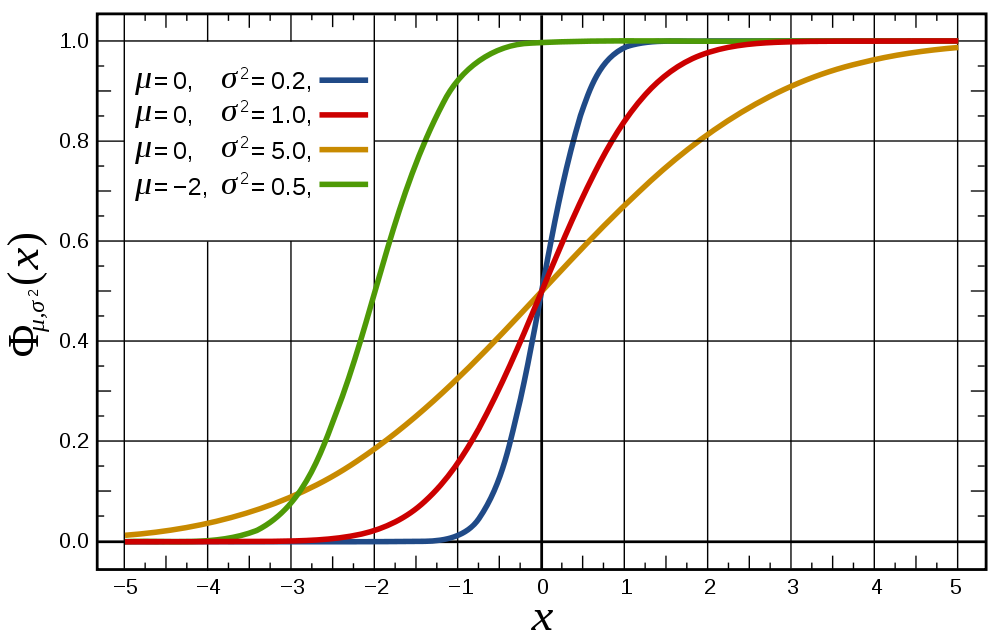
\includegraphics[height=55mm]{pics/cdf_normal.png} &
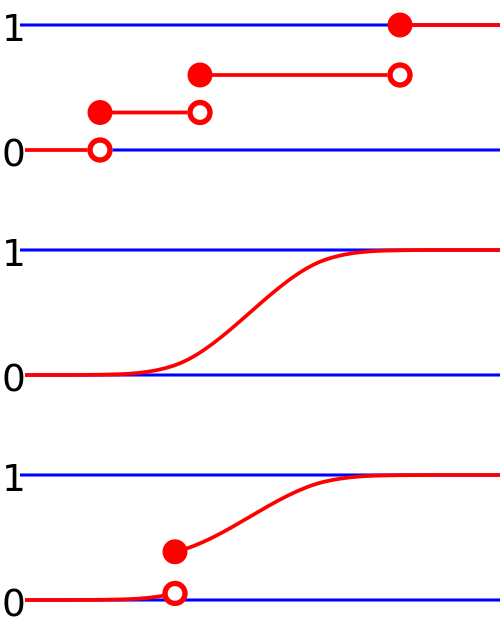
\includegraphics[height=55mm]{pics/cdf_discrete.png}
\end{array}$
\end{center}
\caption{On the left, various normal CDFs. On the right, examples of a discrete, continuous, and a discrete-and-continuous CDF.}
\end{figure}


The probability density function (pdf) of a continuous random variable $X$
is the function $f_X$ that satisfies:

\begin{equation}
	\int_{-\infty}^x  f_X(t)\,\mathrm{d}t = F_X(x) 
\end{equation}

Intuitively, $f_X$ is the simply the probability of $x$ occurring for any given point, (but since $X$ is a continuous random variable, the probability of x occurring at any one point is zero). For discrete random variables, $f_X$ is the function which outputs the probability that $X$ will $= x$ for any input $x$, and it (similarly) satisfies $\sum_{-\infty}^x  f_X(t)\,\mathrm{d}t = F_X(x) $.) 
\\\\
Note that $\sum_{-\infty}^\infty f_X(t)\,\mathrm{d}t = 1 = \int_{-\infty}^\infty f_X(t)\,\mathrm{d}t$.
\\\\
For continuous random variables:
\begin{enumerate}
\item $p(X=x) = 0$
\item $p(X \in A) = \int_{A} f_X(t)\, \mathrm{d}t$
\item $\frac{d}{dx} F_X(x) = f_X(x)$
\item $p(a \leq X \leq b) = p(a < X < b)$
\item This is all just simple calculus stuff.
\\
\end{enumerate}







\section{Moments: mean and variance}
The \textbf{expected value} of a random variable is:\\
$ \sum_{x} xf_X(x)$ \hspace{10 mm}   \dots \hspace{10 mm}   if x is discrete \\
$ \int_{-\infty}^{\infty} xf_X(x)\, \mathrm{d}x $
  \hspace{4 mm}   \dots \hspace{10 mm}  if x is continuous
  \\\\
For integer $n$, the $n^{th}$ moment of $X$ is $E[X^n]$, and the $n^{th}$ central moment of $X$ is $E[(X-E[X])^n]$. 
\\\\
The \textbf{variance} of a random variable is its second central moment,
$E[(X-E[X])^2]$. In Bayesian statistics, the variance of an unknown parameter is the \textbf{uncertainty in belief} of its value.
\\\\
\begin{equation}
E[aX + b] = aE[X] + b 
\end{equation}
\begin{equation}
Var(aX + b) = a^2Var(X) \\
\end{equation}






\section{Likelihood Function}
Let $\textbf{X} = (X_1, X_2, \dots, X_n)$ denote data and $\theta$ denote the unknown parameter(s) of the distribution that defines $X$.
\\\\
Then the \textbf{likelihood function} is the joint pmf/pdf of the data, given the parameters:
\begin{equation}
f(\textbf{X}|\theta) = \prod_{i=1}^n{f(X_i |\theta)}
\end{equation}
But it's often handy to work with the \textbf{log likelihood}:
\begin{equation}
log(f(\textbf{X}|\theta)) = \sum_{i=1}^n log(f(X_i |\theta))
\end{equation}




\section{Maximum Likelihood Estimation}
The maximum likelihood estimator (MLE), $\theta$, maximizes $f(\textbf{X}|\theta)$ to find an estimate of $\hat \theta$: the MLE of $\theta$. 
\\\\
The MLE is asymptotically normal as $n \rightarrow \infty$, with mean 0.
\\


\section{Joint distributions}
$(X,Y)$ is a discrete bivariate random vector if it takes a
countable number of possible values. Then $f_{X,Y}(x,y) = p(X = x, Y = y)$ is the \textbf{joint probability mass
function} of $(X,Y)$, and the \textbf{marginal pmf} of $X$ can be computed as
\begin{equation}
f_X(x) = \sum_{y}f_{X,Y}(x,y)
\end{equation}
\dots where the sum is taken over the values of y such that
$f_{X,Y}(x,y) > 0$.
\\\\
Similarly, $(X,Y)$ is a continuous bivariate random vector if it takes an
infinite number of possible values. Then $f_{X,Y}(x,y)$ is the \textbf{joint probability density
function} of $(X,Y)$ where for every A $\subset \mathbb{R}^2$:
\begin{equation}
	p((X,Y) \in A) = \int \int_{(x,y) \in A} f_{X,Y}(x,y) dx dy
\end{equation}

Then the \textbf{marginal pdf} of $X$ can be computed as
\begin{equation}
f_X(x) = \int_{-\infty}^{\infty} f_{X,Y}(x,y) dy
\end{equation}

These ideas extend to n-dimensional random vectors with $n>2$. 
\\



\section{Conditional distributions \& independence} 

Take a discrete random variable $(X,Y)$: For any $x$ such that $p(X = x) > 0$, the $\textbf{conditional pmf of Y given that X = x}$ is defined as: 

\begin{equation}
f_{Y|X}(y|x) = p(Y=y | X=x) = \frac{p(X=x, Y=y)}{p(X=x)}  =
\frac{f_{X,Y}(x,y)}{f_X(x)}
\end{equation}

Continuous random variable $(X,Y)$: For any set $x$ such that $f_X(x) > 0$, the $\textbf{conditional pdf of Y given that X = x}$ is defined as: 

\begin{equation}
f_{Y|X}(y|x) = \frac{f_{X,Y}(x,y)}{f_X(x)} = \frac{joint(x,y)}{marginal(x)} 
\end{equation}

$X$ and $Y$ are independent if for every $x \in \mathbb{R}$ and $y \in \mathbb{R}$:
\begin{equation}
f_{X,Y}(x,y) = f_X(x)f_Y(y)
\end{equation}




\section{Important Probability Distributions}
\textbf{Discrete}: Discrete Uniform, Binomial, Poisson, Multinomial,
Negative binomial, Hypergeometric
\\
\textbf{Continuous}: Uniform, Exponential, (glorious) Normal, Beta, Gamma,
Inverse Gamma, t
\\




\section{Bayes' Theorem}
By the definition of conditional probability:
\begin{equation}
f(y|x)f(x) = f(x,y) = f(x|y)f(y)  \Longrightarrow f(y|x) = \frac{f(x|y)f(y)}{f(x)}
\end{equation}

Bayes Theorem is central to Bayesian statistics because it allows
us to obtain a posterior for some parameter, given data \textbf{x}:
\begin{equation}
\textit{posterior}(\theta) = f(\theta|\textbf{x}) = \frac{f(\textbf{\textbf{x}}|\theta)f(\theta)}{f(\textbf{x})} \propto f(\textbf{x}|\theta)f(\theta)
\end{equation}

since the denominator, $f(x)$, does not involve $\theta$ in any way, and so is a constant. 
\\\\
Note that we can also rewrite $f(x)$ (by the Law of Total Probability):
\begin{equation}
f(y|x) = \frac{f(x|y)f(y)}{\sum_{y}f(x|y)f(y)} \hspace{10 mm} (discrete \  case)
\end{equation}
\begin{equation}
f(y|x) = \frac{f(x|y)f(y)}{\int_{y}f(x|y)f(y)dy} \hspace{10 mm} (continuous \ case)
\end{equation}



\section{Vocab Review}

{\renewcommand{\arraystretch}{3}
\begin{tabular}{|c|p{10cm}|}
\hline

{\color{red}{Bayes Theorem}} & \rr $f(\theta|\textbf{x}) = \frac{f(\textbf{\textbf{x}}|\theta)f(\theta)}{f(\textbf{x})} \propto f(\textbf{x}|\theta)f(\theta)$ \tn
	 \hline
{\color{red}{Conditional Probability}} & $f(y|x)f(x) = f(x,y) = f(x|y)f(y) $
	\\ \hline
{\color{red}{Marginal Probability}} & $f_X(x) = \sum_{y}f_{X,Y}(x,y)$ \ \ \ OR \ \ \ $\int_{-\infty}^{\infty} f_{X,Y}(x,y) dy$
	 \\ \hline
{\color{red}{Likelihood Function}} & $f(\textbf{X}|\theta) = \prod_{i=1}^n{f(X_i |\theta)}$
	 \\ \hline
\end{tabular} }



\vspace{60mm}

\begin{center}
\textit{Okay, that's it for review. Now go drink a glass of orange juice. Or be a beast and read on immediately. When you do read on, though, try to work out stuff on paper if you don't grasp it. Or use google. Or whatever.}
\end{center}






\chapter{The Story: Likelihoods, Priors, and Posteriors}
\begin{enumerate}
\item \textbf{Wait, what?}
\item \textbf{Bayesian Inference}
%\item \textbf{Proirs, Posteriors, and Conjugacy}
%\item \textbf{Inference Via Simulation}
\item \textbf{Hierarchical Models}
\end{enumerate}

\vspace{10 mm}

\section{Wait, what?}
So, we have this Bayes equation. But what the hell is $p(data|\theta),  p(\theta)$, or $p(data)$, in the equation:

\begin{equation}
f(\theta|\textbf{data}) = \frac{f(\textbf{\textbf{data}}|\theta)f(\theta)}{f(\textbf{data})} \propto f(\textbf{data}|\theta)f(\theta)
\end{equation}
Well,
  \begin{enumerate} 
          \item $p(data|\theta)$ is simply the likelihood (the `L' in the MLE Maximum Likelihood Estimate) of your data given $\theta$. So, for observed data $x_i$...$x_n$, we have: 
          \begin{equation}
          \prod\nolimits_{i=1}^n f(x_i|\theta)
          \end{equation}
          \item $p(data)$ is just a constant, so in practice we can just ignore it, and then make sure our resultant equation $p(\theta|data)$ sums to 1, since $p(\theta|data)$is a probability distribution. (It's a constant because it doesn't involve $\theta$, which is the variable we're looking at in $p(\theta|data)$.)
         \item  $p(\theta$) is a \textbf{prior distribution} that you may pick based on prior data or beliefs, before looking at your data $X$. Often, when you really don't have an idea of what $\theta$ is, you can choose a non-informative prior (more on this later - if you're a bit confused, no worries).
           \end{enumerate}


\section{Bayesian Inference}
In Bayesian Statistics, the story is basically this:
\\\\
{\color{violet}{
 We have some data \textbf{x}, and we want to fit a good model to it, generally either to be able to predict new future data or explain the past better. So first, we choose some model M (e.g. a binomial model for coin flips), and define our prior beliefs about the model M's parameter(s), $\theta$ (e.g. I think that the coin has a 50\% chance of being fair: $\theta$=.5, and a 25\% chance each of $\theta$ being .2 or .8). 
\\\\
Then we calculate the posterior distribution of $\theta$, given our prior beliefs, our chosen model, and the data \textbf{x} that we have using Bayes Rule:
\begin{equation}
f(\theta|\textbf{x}) \propto f(\textbf{x}|\theta)f(\theta)
\end{equation}
\begin{equation}
posterior \ \propto \ likelihood \ *\ prior
\end{equation}

Using this posterior distribution of $\theta$, we can now predict new values of \textbf{x}: 
$\widetilde{\textbf{x}}$, by determining $p(\widetilde{\textbf{x}} | $ \textit{info \& assumptions \& past data}$)$:
\begin{equation}
p(\widetilde{\textbf{x}}|\textbf{x}) = \int p(\widetilde{\textbf{x}}|\theta)p(\theta|\textbf{x}) d\theta
\end{equation}

 From this, we can really make any type of inference about future data values, assuming our model is correct (e.g. confidence intervals, means, etc...). But is the model correct? That's the last part of the story. Model checking and model comparison! Basically, say you've done the above process with a few different priors, and even a few different models (perhaps a hypergeometric instead of binomial model, or with a `hyper'-prior on the parameters of your original prior). How do you know: 1) if a model makes sense, and is good, and 2) which of many models is best. To roughly determine which model looks best, often people use what's called a \textbf{Bayes Factor}:
 \begin{equation}
B_{12}= \frac{p(\textbf{x}|M_1)}{p(\textbf{x}|M_2)}
\end{equation}

Where $M_i$ = Model $i$. But with many models, it's generally just `who has the highest $p(\textbf{x}|M_i)$'. Model checking will be discussed later on, but basically, you simulate k sets of length n values of $\widetilde{\textbf{x}}$, calculate k test statistics (e.g. mean, sd, min, max), and check to see if the test statistic calculated from your data $\textbf{x}$ is not an extreme value when compared to the distribution of k-test statistics that you have calculated from simulated values.
}}
\\\\
Below, you'll find a basic scenario in theory on the left, with an example of each step with real data on the right.
\\\\
\twocolumn 
\begin{enumerate}
\item Specify a likelihood distribution and a prior \textit{before} inspecting your data. If you let your data $x$ influence your prior(s) in any significant way, you'll end up over fitting, and your resultant $\theta$ confidence intervals will be tighter than they should be. This is especially important when you don't have a lot of data, because your prior(s) will have a stronger influence on your posterior distribution(s).
\item Collect some data, $\textbf{x}$.
\item Compute the posterior distribution for the parameter(s) of interest, $\theta$, given the particular $\textbf{x}$ that you saw: $f(\theta|\textbf{x})$.
\item Make statistical inferences about your posterior distribution, about your model, and about future predicted data (you'll see that this is quite easy once you have (c).
\item Model Check. (Posterior Predictive Checks)
\item If model checking resulted in depression and despair at your future statistical success, repeat steps 1-5 again. Possibly use Bayes Factor to compare multiple models.
\item Refuse to get a job as an investment banker.
\end{enumerate}
{\color{blue}{
\begin{enumerate}
\item 
\item 
\item 
\item 
\item 
\item 
\end{enumerate}
}}
\newpage

\onecolumn

%
%\section{Priors, Posteriors, and Conjugacy}
%Calculating this stuff is not always so easy, though. But there are some tricks. A conjugate prior for some likelihood is a prior such that when used as a prior on the given likelihood, the posterior distribution is in the same family as the conjugate prior. So:
%\begin{equation}
%f(\theta|\textbf{x}) \propto f(\textbf{x}|\theta)*prior
%\end{equation}
%You may choose prior \textbf{hyper parameters} (the parameters of your prior distribution(s) based on your prior beliefs about the parameter your prior defines. For example, if your prior is from the Normal family, but you really know nothing about it, you can create a \textbf{non-informative prior} by giving your prior a variance of $\infty$.
%
%\begin{adjustwidth}{2em}{0pt}
%{\color{blue}{
%\vspace{10mm}
%\textbf{EXAMPLE:} to come. Probably exponential. That's easyish.
%\vspace{10mm}
%}}
%\end{adjustwidth}
%
%
%
%\section{Inference via simulation}
%Simulation is a central part of applied Bayesian analysis. We can often generate samples from a distribution even if its pdf cannot be integrated (giving us an easier way to estimate integrals). Using the badass power of computers, simulation is often straightforward.
%
%



\section{Hierarchical Models}

Okay, that's great and all, but it's hard to see why this is so much more powerful than classical frequentist statistical inference. Well, one of the strengths of Bayesian Analysis is that it's not to hard to build quite complex, hierarchical models.

\begin{center}
% The state vector is represented by a blue circle.
% "minimum size" makes sure all circles have the same size
% independently of their contents.
\tikzstyle{blue}=[circle,
                                    thick,
                                    minimum size=1.2cm,
                                    draw=blue!80,
                                    fill=blue!20]

% The measurement vector is represented by an orange circle.
\tikzstyle{yellow}=[circle,
                                                thick,
                                                minimum size=1.2cm,
                                                draw=orange!80,
                                                fill=orange!25]

% The control input vector is represented by a purple circle.
\tikzstyle{red}=[circle,
                                    thick,
                                    minimum size=1.2cm,
                                    draw=purple!80,
                                    fill=purple!20]

% The input, state transition, and measurement matrices
% are represented by gray squares.
% They have a smaller minimal size for aesthetic reasons.


\tikzstyle{whitespace}=[rectangle,
                                    thick,
                                    minimum size=1.1cm,
                                    draw=white!80,
                                    fill=white!20,
                                    ]


\begin{tikzpicture}[>=latex,text height=1ex,text depth=0.25ex]
    % "text height" and "text depth" are required to vertically
    % align the labels with and without indices.
  
  % The various elements are conveniently placed using a matrix:
  \matrix[row sep=0.45cm,column sep=.25cm] {
    % First line
    &
        \node (whitespace)   [whitespace] {};       &
        \node (whitespace)   [whitespace] {};       &
        \node (normal-2)   [red]{$\beta$ Normal};     &
        \\
		\\
        % Second Line
        \node (whitespace)   [whitespace] {};       &
        \node (th1) [blue] {$\mathbf{\theta}_{1}$}; &
        \node (A_k-2)         {$\cdots$};           &
        \node (th2)   [blue] {$\mathbf{\theta}_i$};     &
         \node (A_k-2)         {$\cdots$};           &
        \node (th3) [blue] {$\mathbf{\theta}_{n}$}; &
        \\
        % fourth line
        &
        \node (x1) [yellow] {$\mathbf{X}_{1}$}; &
          \node (A_k-2)         {$\cdots$};           &
        \node (x2)   [yellow] {$\mathbf{X}_i$};     &
          \node (A_k-2)         {$\cdots$};           &
        \node (x3) [yellow] {$\mathbf{X}_{n}$}; &
        \\
    };
    
    % The diagram elements are now connected through arrows:
    \path[->]

        (normal-2) edge (th1)			
        (normal-2)  edge (th2)
        (normal-2)  edge (th3)

        (th1) edge (x1)
        (th2) edge (x2)
        (th3) edge (x3)
        ;
 
\end{tikzpicture}
\end{center}



(1) was used for prior probabilities, and the estimation of prior hyper-parameters. (3) was used to create 0-1 polling-like data from (2). The 0-1 data was used to estimate the posterior probability of each state's vote-share, which was then used to estimate the posterior probability of Obama winning the election.



\section{Multi-Parameter Bayesian Models}
Thus far, we have seen Bayesian inference in single-parameter
models. Most real problems require multiple parameters to
appropriately model the data. Example: Regression problems with multiple covariates. Advantages to the Bayesian approach to inference stand out in higher-dimensional problems.
\\\\
Bayesian tools allow us to marginalize over the values of
unknown nuisance parameters to obtain posterior distributions
over the parameter(s) of interest:
\begin{equation}
p(\theta_1|\textbf{x}) = \int p(\theta_1, \theta_2|\textbf{x}) \ d\theta_2
\end{equation}
... where $p(\theta_1, \theta_2|\textbf{x}) \propto p(\textbf{x}|\theta_1, \theta_2)p(\theta_1, \theta_2)$.




\section{Vocab Review}

{\renewcommand{\arraystretch}{2.7}
\begin{tabular}{|c|p{10cm}|}
\hline

{{Bayes Theorem}} & \rr $f(\theta|\textbf{x}) = \frac{f(\textbf{\textbf{x}}|\theta)f(\theta)}{f(\textbf{x})} \propto f(\textbf{x}|\theta)f(\theta)$ \tn
	 \hline
{{Conditional Probability}} & $f(y|x)f(x) = f(x,y) = f(x|y)f(y) $
	\\ \hline
{{Marginal Probability}} & $f_X(x) = \sum_{y}f_{X,Y}(x,y)$ \ \ \ OR \ \ \ $\int_{-\infty}^{\infty} f_{X,Y}(x,y) dy$
	 \\ \hline
{{Likelihood Function}} & $f(\textbf{X}|\theta) = \prod_{i=1}^n{f(X_i |\theta)}$
	 \\ \hline
{\color{red}{$p(data|\theta)$}} & The likelihood of your data, given parameter(s) $\theta$: $\hspace{30mm}$ $f(\textbf{X}|\theta) = \prod_{i=1}^n{f(X_i |\theta)}$
	\\ \hline
{\color{red}{Prior Distribution}} & $p(\theta)$ \dots \ The distribution from which your (model assumes) parameters are pulled. e.g. The distribution from which $\theta$ is pulled, where the distribution from which each $X_i$ is determined by the value(s) of $\theta$.
	 \\ \hline
{\color{red}{Hyperparameter}} & $\alpha$ \dots \ A parameter that defines the distribution of your prior distribution. e.g. a hyper parameter $\alpha$ that defines the distribution from which $\theta$ is pulled, which then defines the distribution from which each $X_i$ is pulled (according to the model).
	 \\ \hline
\end{tabular} }




\chapter{Priors}
\section{What is a Prior?}
Philosophically, what is a prior? \\
- non informative priors (Why can't you just use 1? In some cases, I'm not even entirely sure.)\\  
- informative priors (Only use these when you \textit{are} informed)\\
\\\\
Informative Priors:\\
\textbf{State of Knowledge Interpretation}: We express all knowledge
and uncertainty about $\theta$ (prior to collecting data) as if its
value could come from a random draw from the prior, $p(\theta)$
\\
\textbf{Population Interpretation}: The prior distribution represents a
population of possible parameter values, from which the $\theta$ of
current interest is drawn.
\\\\
You don't have to worry excessively about getting your prior exactly right when you're going to have a lot of data, because as more data is incorporated into the equation, the prior matters less and less (the weight of the data overpowers it). In my opinion, it is good practice to overestimate the variance on your priors, if your priors are coming from your gut, as opposed to another source of data (like history). (So, e.g., you could assume a normal distribution over some prior parameter $\theta$ with variance 10, or variance 15, the latter being `safer'.) If you don't have a lot of data, and your prior is unjustly narrowly centered around your data, you'll be over-fitting.


\section{Conjugate Priors}

So, we have our handy dandy Bayes equation:

\begin{equation}
f(\theta|\textbf{x}) \propto f(\textbf{x}|\theta)f(\theta)
\end{equation}

... where our data is represented by $\textbf{x}$. And we want to know the left side of the equation, the posterior distribution. Well, with certain assumed priors and data likelihoods, this is not so difficult. Others result in scary integrals that are literally un-integratable, which you'll need a computer (or 674 pencils) to solve well. We're going to start with the nice situations first, that don't require computers. Yay, us. These easy situations arise when your prior is `conjugate' to your data's likelihood distribution (i.e. the type - normal, exponential, beta, etc., not its parameters).
\\\\
With a conjugate prior, the posterior generally just pops out of the above equation when you plug everything in and sort some things out, and that posterior distribution will be from the same type of distribution as the prior (e.g. exponential, beta, etc..., but with slightly different parameters to take into account your data, $\textbf{x}$). Computations of the posterior with a conjugate prior are pretty easy to do.


\begin{adjustwidth}{2em}{0pt}
{\color{blue}{
\vspace{10mm}
\textbf{EXAMPLE:} to come.
LIST OF CONJUGATE PRIORS and LIKELIHOODS to come.
\vspace{10mm}
}}
\end{adjustwidth}


Often, a distribution's conjugate prior often is flexible enough to approximate a large number of prior beliefs. As we collect even more data (under the same likelihood), the posterior can be used as the next prior and it will be conjugate! This allows for easy updates.
\\\\
However, with some likelihoods, conjugacy does not exist,
especially in multi-dimensional parameter spaces. Additionally, some likelihood's conjugate priors will not be able to describe your prior beliefs well, in which case you'll need to use non-conjugate priors and more advanced methods.
\\\\
Note that all likelihoods from the exponential family have conjugate priors. These include: normal, exponential, gamma, beta, Bernoulli, Poisson, etc.
\\\\
When you have a conjugate prior, you can literally just plug in your information into the equation ...
\begin{equation}
f(\theta|\textbf{x}) \propto f(\textbf{x}|\theta)f(\theta)
\end{equation}
... to get $f(\theta|\textbf{x})$.
\\\\
A prior can express specific prior information about parameters.\\
- That the parameter is known to fall in some subspace (e.g. some proportion in [0,1]).\\
- Knowledge gained from previous experiments.\\
- Opinions from experts in the field (generally unsubstantiated with data that can be integrated into the model). 
\\\\
Generally, the more data a model is given, the less influence the prior will have on the final posterior estimation. So when you have a lot of data, it's less important to perfectly represent your prior, but it \textit{is} always extremely important to make sure your prior probabilities are non-zero at any values that your parameter $\theta$ may take!




\section{Non-Informative Priors}
A prior can also express a lack of information. When little information about a parameter $\theta$ is known before looking at the data, it's important to use a non-informative prior, whose goal is basically to have a minimal impact on the posterior - let the data speak for themselves.
\\ 
- We can use high variance priors if we have little confidence about our prior beliefs. \\
- Non-informative priors are great if we have no prior beliefs and/or do not want to influence the analysis with a prior.


\begin{adjustwidth}{2em}{0pt}
{\color{blue}{
\vspace{10mm} 
\textbf{EXAMPLE:} \textit{Non-informative Prior for Binomial Likelihood} \\
If $\textbf{X}|\theta \sim Binomial(n, \theta)$, then \\
$\theta \sim Uniform[0,1]$ is non-informative because \\
$ p(\theta|\textbf{X} \propto p(\textbf{X}|\theta)p(\theta) = p(\textbf{x}|\theta)$
\vspace{10mm}
}}
\end{adjustwidth}


Principle of Indifference: All values are equally likely a priori. The simplest type of non-informative prior is a prior which is flat across its parameter space.
\\
An improper prior does not integrate to 1. 
\\\\
The problem with flat priors... (--$>$ Jeffrey's Prior).
\\\\
- transformations of random variables



\section{Well, Shit}
In the previous section, we were able to use handy priors and likelihoods to calculate posterior distributions by hand. But - come on, it's usually not going to be the case that the data and story that you're looking at are represented ideally by a conjugate prior and likelihood pair. 
\\\\
Solution? Glorious computers, that's what.







\chapter{Grid Approximation}
So, faced with both a computer, and an ugly non-conjugate problem, or a conjugate problem plus laziness, grid approximation is the most intuitive thing to do. It goes like this: instead of having an equation representing the prior probability for any value of $\theta$, you can have a vector of actual $\theta$ values, and corresponding probability vector of the same length, where each element $i$ in this probability vector is the probability that element $i$ in the $\theta$ vector will occur, of all the $\theta$ given. 



\begin{adjustwidth}{2em}{0pt}
{\color{blue}{
\vspace{10mm} 
\textbf{EXAMPLE:} to come.
\vspace{10mm}
}}
\end{adjustwidth}



So. That's awesome and simple and intuitive. My kind of thing! But, wait, theeeeere's less! Grid approximation does not do so well in high dimensional problems. Say you have ten different parameters that affect your final posterior distribution: in order to maintain grid close-ness in your ten-dimensional sample space, the fineness of your grids will have to grow exponentially! If your initial parameter was defined over $[0,1]$ and you had $100$ equally spaced samples, to keep that fineness in the ten-dimensional parameter space, you'd now need $100^{10}$ samples! ($100,000,000,000,000,000,000$, or $1e+20$.)
\\\\
Another problem is non-smooth distributions. If your priors are particularly bumpy, grid approximation might not work well.
\\\\
\begin{figure}[h]
\begin{center}$
\begin{array}{cc}
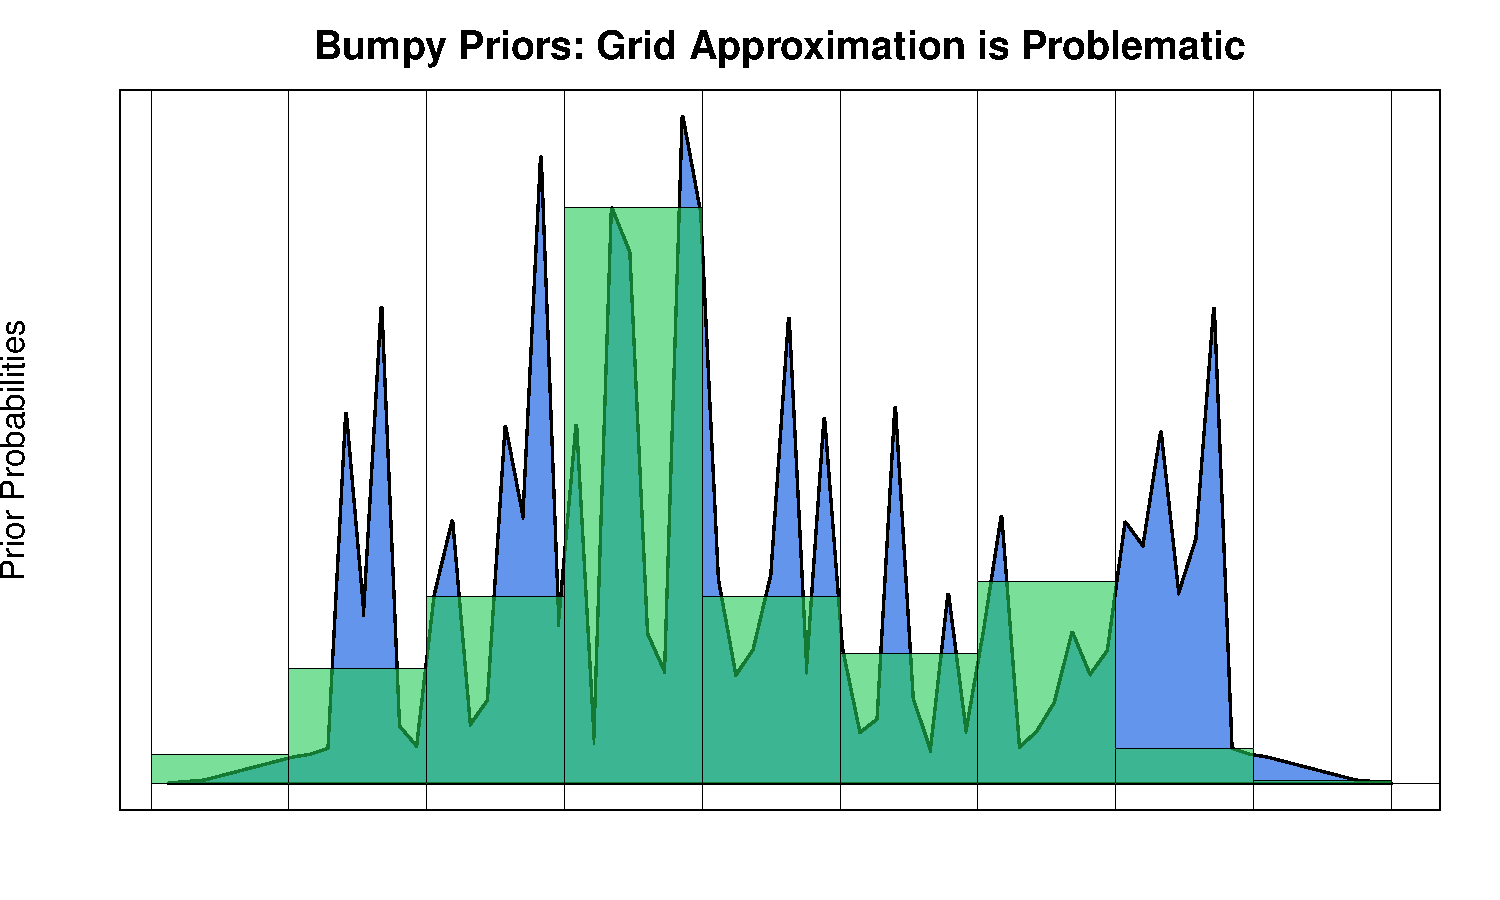
\includegraphics[height=75mm]{pics/bumpy.pdf} 
\end{array}$
\end{center}
\caption{An exaggeration of how a `bumpy' distribution may not be well estimated by a grid approximation.}
\end{figure}
\\\\
But, worry not - there are yet cooler methods of estimating the posterior distribution of a parameter $\theta$ with good 'ol computers.






\chapter{Model Checking \& Model Comparison}


\chapter{Bayesian Sampling}
This chapter deals with with situations when it's either impossible or just not easy to calculate a posterior distribution, and for whatever reason (high dimensionality, bumpy priors, or needed accuracy) grid approximation is not optimal. The following sections outline various algorithms and methods to sample from such posterior distributions.


\section{Rejection Sampling}
Say that you have a positive function $f(\theta)$ from which we want to draw samples. Unfortunately, you don't know how to draw samples from it. But you do know how to draw samples from another density $g(\theta)$, where $g(\theta)$>0 for each $\theta$ where $f(\theta) > 0$.

\begin{enumerate}
\item Find a number M such that $\frac{f(\theta)}{g(\theta)} \leq M \ \ \forall \theta$.
\item Generate a number $\theta$ from $g()$.
\item Generate a number $u$ from Uniform[0,1].
\item If $u \leq \frac{f(\theta)}{Mg(\theta)}$ then accept $\theta$ as a pull from $f()$.
\item Repeat 2-4 until you have enough samples!
\end{enumerate}


Note that, for efficiency's sake, you want $f$ and $Mg$ to be as close as possible, so you end up rejecting as few $\theta$ as possible.
One easy approach is to just set $g(\theta)$ equal to your prior, $p(\theta)$, so that:
\begin{equation}
\frac{f(\theta)}{g(\theta)} = \frac{p(\textbf{x}|\theta)p(\theta)}{p(\theta)} = p(\textbf{x}|\theta) \leq p(\textbf{x}|\hat \theta_{MLE}) = M
\end{equation}
This approach is a good one, although sometimes it is inefficient if $g = Mp(\textbf{x}$ is far above $f(\theta)$ in most places. Additionally, M is not always easy to find. In which case, other approaches may be used...

\section{Sampling Importance Resampling (SIR)}
Sampling Importance Resampling is very similar to Rejection Sampling. Again, you start off with a function $f(\theta)$ that you can't pull samples from, and a function $g(\theta)$ such that $f(\theta) \leq g(\theta)$ for all $\theta$. Then:
\begin{enumerate}
\item Draw a sample $\theta_1,\dots, \theta_n$ from $g$.
\item For each $\theta$, calculate $w_i = \frac{f(\theta)}{g(\theta}$
\item Calculate $q_i = \frac{w_i}{\sum_iw_i}$
\item Draw, with replacement, from $\theta_1,\dots, \theta_n$ with probability $q_i$ for each $\theta_i$
\end{enumerate}
The sample that you get is pretty much equivalent to a draw from $f$, especially when $n$ is large and $f$ and $g$ are relatively `non-bumpy'.

\section{MCMC Methods}
Markov Chain Monte Carlo methods are a set of stochastic methods that are great for sampling from difficult target distributions. They're useful in high dimensional problems (e.g. 100 different $\theta$s), when conjugacy does not hold and grid approximations are not useful. MCMC methods are iterative - they basically loop around some list of rules (algorithm) to eventually develop a posterior distribution. Three are three popular versions: Gibbs Sampling, Metropolis Hastings, and Metropolis. 

	\subsection{Markov Chain}
	A Markov chain is a process $X_t = X_0, X_1, \dots, X_T$ in discrete time $t=0,1, \dots,T$ where $p(X_t|X_0, X_1, \dots, X_{t-1}) = p(X_t|X_{t-1})$. In other words, $X_t$ is only affected by the last $X_{t-1}$, but not by any other previous $X$s. (Comparing this to Poisson's `memoryless' attribute, you can think of Markov Chains as having very short term memories! Uhhh, \textit{50 First Dates}, anyone?)
	\\\\
	A Markov chain is \textbf{irreducible} if it is possible to reach all states (all possible `$X$'s) from any other state. So, if $p^n(j|i)$ represents the probability of getting from state $i$ to state $j$ in $n$ steps, then irreducibility means that for any $i$ and $j$, 
	\begin{equation}
	p^n(j|i) < 0 \ \textnormal{and} \ p^m(i|j) < 0 \ \textnormal{for some m, n}
	\end{equation}
	
	A Markov chain is \textbf{periodic} with period $d$ if $p^n(i|j) = 0$ unless $n=kd$ for some integer $k$. If $d=1$ then chain is \textbf{aperiodic}. 
	\\\\
	\begin{adjustwidth}{2em}{2em}
\textbf{THEOREM}: A finite-state, irreducible, aperiodic Markov chain has a limiting stationary distribution: $\pi = lim_{n \to \infty}p^n(j|i)$. Then the limiting distribution, $\pi$, is reached no matter where we start the Markov chain. \\\\ 
	\end{adjustwidth}
	The idea behind Markov Chain Monte Carlo methods is the following: you want to sample from some posterior distribution, $p(\theta|\textbf{x})$, but it's too difficult, so instead you create a Markov Chain ${\theta(t), t \in T}$, with a stationary distribution $p(\theta|textbf{x})$. In other words, as $t \to \infty$, then the samples given by the Markov Chain will be equivalent to samples taken from our wanted posterior distribution, $p(\theta|\textbf{x})$.
	\\\\
	In this scenario, we know the stationary distribution we want - $p(\theta|\textbf{x})$ - and we want a Markov chain that will take us there: $\pi = p(\theta|\textbf{x})$ as $t \to \infty$. Once you find that chain, all you have to do is choose some initial value(s) $\theta$ and run the chain for a large number of steps until it \textit{converges} to $\pi$ (more on how to tell if it's converged later).  Then you can run it for a large number of more steps to get decent `pull' from our wanted posterior distribution.
	\\\\
	All MCMC methods stem from this idea. The only difference is how the Markov chain transitions are made. Some algorithms are less prone than others to getting `stuck' on a probability hill (local modes in the density curve of your posterior distribution), while some take longer to converge.
\\\\
	But, question: how the hell are you supposed to create out of thin air a Markov Chain like that? Well, the short answer is that you don't really have to. There are a lot of cool, free, and easy programs you can use (e.g. packages in R) that do it for you. But, we'll go over the theory anyways, and then some computer examples using R.
	\\\\
	\subsection{Gibbs Sampling}
	A Gibbs Sampler is an MCMC algorithm that uses conditional posterior distributions, $p(\theta_i|\theta_1,\dots, \theta_{i-1}, \theta{i+1},\dots, \theta_n, \textbf{x}) = p(\theta_i|rest, \textbf{x})$, to develop the wanted posterior distribution, $p(\theta|\textbf{x})$. All $i$ conditional posterior distributions are cycled through for each iteration of the Gibbs sample. 
	Say that you have three parameters $\theta = \theta_1, \theta_2, \theta_3$. To begin a Gibbs Sampler, you first have to guess initial values $\theta^0 = \theta^0_1, \theta^0_2, \theta^0_3$. Then one iteration of the Gibbs Sampler is as follows:
	\begin{enumerate}
	\item Draw $\theta_1^1$ from $p(\theta_1|\theta_2 = \theta_2^0, \theta_3 = \theta_3^0, \textbf{x})$
	\item Draw $\theta_2^1$ from $p(\theta_2|\theta_1 = \theta_1^0, \theta_3 = \theta_3^0, \textbf{x})$
	\item Draw $\theta_3^1$ from $p(\theta_3|\theta_1 = \theta_1^0, \theta_2 = \theta_2^0, \textbf{x})$
	\end{enumerate}
	So you get $\theta^1 = \theta^1_1, \theta^1_2, \theta^1_3$, which you can use to replace $\theta^0$ with, to then repeat steps 1-3 again, for a second iteration of the sampler. And so on and so forth, until you have converged your sampler, and later have a nice sample of $\theta$s from your wanted posterior distribution, $p(\theta|\textbf{x})$. 
	\\\\
	Note that Gibbs Samplers can be created relatively easily for models that are either conjugate or \textbf{semi-conjugate} (?). A semi-conjugate prior is a prior that is the product of priors:
	\begin{equation}
	p(\mu, \sigma^2) = p(\mu)p(\sigma^2)
	\end{equation}
	... each of which, conditioned on the other parameters, is conjugate. (?)
	\\\\
	When the conditional distributions of a posterior distribution are easy to derive and sample from, Gibbs Sampling is a very efficient method, and it converges quickly. However, conditional distributions are not always easy to derive. Slower, but much more general algorithms like Metropolis Hastings work well in these scenarios.

	\subsection{Metropolis} 
	While Gibbs Sampling requires that we can sample from full conditionals of $p(\theta)$, the Metropolis and Metropolis Hastings algorithms need only our model's likelihood and priors. (Gibbs Sampling is actually a less powerful, special case of the Metropolis Hastings MCMC method.) 
	\\\\
	The Metropolis algorithm (like Gibbs) begins with the selection of initial value(s), $theta^0 = \theta^0_1, \theta^0_2,\dots, \theta^0_n$. Then one iteration of the Metropolis-Hastings algorithm is as follows:
	\begin{enumerate}
	\item Sample a proposal $\theta$ from a proposal (jumping) distribution, $J_t(\theta^*|\theta^{t-1})$. Note that the the proposal distribution must be symmetric, i.e.
	\begin{equation}
	 J^t(\theta_a|\theta_b) = J^t(\theta_b|\theta_a) \ \ \forall \ \theta_a, \theta_b, t
	 \end{equation}
	 
	\item Compute the ratio of the posteriors:
	
		\begin{equation}
			r = \frac{p(\theta^*|\textbf{x})}{p(\theta^{t-1}|\textbf{x})}
		\end{equation}
	
	\item Set the next point ($\theta_i$ in $n^{th}$ dimensional space) in the Markov chain equal to:
		\begin{equation}
\theta^t = \begin{cases}
  \theta^*, & \text{with probability $min(r, 1)$}, \\
  \theta^{t-1}, & \text{otherwise}.
\end{cases}
	    \end{equation}
	\end{enumerate}
	In other words, the Metropolis algorithm always accepts proposals of $\theta^*$ for which $p(\theta^*|\textbf{x}) \geq p(\theta^{t-1}|\textbf{x})$, and we only sometimes accept proposals of $\theta^*$ for which $p(\theta^*|\textbf{x}) < p(\theta^{t-1}|\textbf{x})$, with acceptance probability corresponding to the probability of $p(\theta^*|\textbf{x})$ compared to $p(\theta^{t-1}|\textbf{x})$.
	\\\\
	The result of this is that the Metropolis algorithm doesn't always go uphill, so it won't always get stuck in local probability maxima.
	\\\\
	Although there are various options, the multivariate normal distribution, with a mean of $\theta^{t-1}$, is the most often chosen for $J_t$.
	\\\\
	I'm too lazy to write down the proof, for now.
	
	
	\subsection{Metropolis Hastings}
The Metropolis Hastings algorithm is similar to, but even more flexible than the Metropolis algorithm. The proposal density of the Metropolis Hastings algorithm doesn't need to by symmetric, i.e. $J^t(\theta_a|\theta_b)$ need not equal $J^t(\theta_b|\theta_a)$. But to correct for the asymmetry, the ratio $r$ is replaced by:
	\begin{equation}
			r = \frac{p(\theta^*|\textbf{x}) / J_t(\theta^*|\theta^{t-1})}
			{p(\theta^{t-1}|\textbf{x}) / J_t(\theta^{t-1}|\theta^{*})}
	\end{equation}
Allowing these asymmetric jumps can accelerate convergence.
\\\\
The Metropolis and Metropolis-Hastings algorithms don't require that we can derive the conditional posteriors (as is necessary in Gibbs sampling), but it also means that Gibbs sampling, unlike the Metropolis and Metropolis-Hastings algorithms, requires that we can derive conditional posteriors. However, it has the benefit of never throwing out any proposed points of $\theta$. As a result, Metropolis and Metropolis-Hastings algorithms tends to be much less efficient (slower). 
\\\\
The more narrow your proposal density is, the slower your model will converge. But the wider your proposal density is, the more crazy your proposal $\theta$s will be, leading to a lot of rejection. It's a fine line!
\\\\
An often used proposal density is the multivariate normal with mean $\theta^{t-1}$, but with correlation matrix $\sum$. The optimal proposal covariance is the true covariance of the posterior, but this is unknown, so we have to estimate it, and then adjust it over iterations. (Optimal acceptance rates of proposed values are generally in between 25 and 50\%, although these percentages get smaller for higher dimensional problems). A solid estimate for $\sum$ is the inverse observed Fisher Information matrix. (?)
\\\\
In general, when you're working on problems that don't take hours (or days, months, or years!) to compute, Metropolis and Metropolis-Hastings algorithms are a great, flexible bet (and are particularly easy to use in $R$).

\section{MCMC Diagnostics}
So I've been talking about checking for `convergence' this whole time without really explaining what that means. In a nutshell, as I mentioned before, a model has converged when the samples you are drawing from it are (more or less) equivalent to drawing from the true posterior distribution you are aiming for. As $t \to \infty$, this is guaranteed, but models generally converge much quicker than that, thankfully. But how can you tell? Well, there are both numeric and visual tests you can run to see if your model seems to have converged.
\subsection{Traceplots}
\subsection{Autocorrelation Plots}
\subsection{Multiple Sequence Diagnostic}


\chapter{Linear Models}
Linear modeling is probably the most widely used statistical tool. It's also severely misunderstood by many, but  hey, what to do expect? (A lot of people seem to forget that linear models are just that - \textit{linear}! They only detect linear trends. It's always important to visualize your residuals (data - line) before making any conclusions. But, that's another rant. Additionally, the distance measure that people generally use is not some God-given formula - it's relatively arbitrary, used mostly because of mathematical convenience. But, that's neither here nor there...) The basic question to be answered is this: \textit{how does a an `outcome', $y$, vary with regards to a vector of covariates, $\textbf{x} = x_1, \dots, x_n$?}
\\\\
$\textbf{x}$ and outcome $y$ can be discrete or continuous. The matrix of covariates, $X$, is called the \textbf{design matrix}. The most commonly used linear regression model goes something like this:
	
\begin{equation}
	y_i \sim \beta_1x_{i,1} +  \beta_2x_{i,2} + \dots +  \beta_nx_{i,n}
\end{equation}
\begin{equation}
	\textnormal{error}_i = \epsilon_i \sim \textnormal{Normal}(0, \sigma^2)
\end{equation}

Then the likelihood for the normal linear model is then:

\begin{equation}
	\textbf{y}|\beta \sigma^2, \textbf{X} \sim \textnormal{Normal}(\textbf{X}\beta, \sigma^2 I)
\end{equation}

A handy non-informative prior on $(\beta, \sigma^2)$ is $p(\beta, \sigma^2) \propto \sigma^{-2}$. It's not very hard to derive conditional posterior distributions of $\beta$ and $\sigma^2$, which allows one to use a Gibbs sampler to determine the posterior distribution of \textbf{y}!

\begin{equation}
	\beta| \sigma^2, \textbf{X}, \textbf{y} \sim \textnormal{Normal}\bigg((\textbf{X}^T\textbf{X})^{-1}\textbf{X}^T\textbf{y}, \ \sigma^2(\textbf{X}^T\textbf{X})^{-1}  \bigg)
\end{equation}

\begin{equation}
	\sigma^2|\beta, \textbf{X}, \textbf{y} \sim \textnormal{Inverse-Gamma}\bigg(\frac{n-k}{2}, \frac{n-k}{2}s^2 \bigg)
\end{equation}

It's also nice to be able to predict new value of $\widetilde y$ for a new set of covariates $\widetilde x_1, \dots,\widetilde x_n $, i.e. draw from the posterior predictive distribution: $p(y|\textbf{y}, \textbf{X}, \widetilde x_1, \dots,\widetilde x_n)$



	\section{Simple Linear Models}
	\section{Hierarchical Linear Models}



A \textbf{Simple Random Effects Model} is a linear model that may be described as follows:
\begin{equation}
y_i|\beta, \sigma^2, \textbf{x}_i \sim \textnormal{Normal}(\beta_0 + \beta_{1} x_{i,1} + \dots + \beta_{p} x_{i,p}, \sigma^2 )
\end{equation}
Where
\begin{equation}
\beta_j \sim \textnormal{Normal}(\alpha, \sigma^2_\beta) \ for \ j \in 0, ... , p
\end{equation}
Example: \\
$x_{i,j} = I(student \ i \ is \ in \ school \ j)$
(Where $I$ is an indicator function.) Each school has its own effect on student performance, $y_i$, but the schools are all tied together via the common prior over $\beta_1, ..., \beta_p$.
\\\\
A \textbf{Mixed Effects Model} is a linear model where: \\
\hspace{10 mm} $\beta_1, ..., \beta_m$ have independent non-informative priors (`fixed effects'), and \\
\hspace{10 mm} $\beta_m+1, ..., \beta_p  \sim \textnormal{Normal}(\alpha, \sigma^2_\beta)$ (`random effects').

The term random effects refers to the deviations of randomly-selected entities (e.g., schools) from the average.
When dealing with lots of predictor variables (large p), usually
most of them will have no effect $(\beta = 0)$
\\\\
In classical statistics, there are many methods to try to select a
subset of covariates: forward / backward stepwise selection,
least-angle regression, Lasso, ridge regression ,etc.

In Bayesian Regression, we can achieve similar results using
hierarchical linear models by setting up a prior distribution over the
$\beta$ parameters that gives each parameter a high probability of being near zero and a small probability of being far from zero


\chapter{Bayesian Model Averaging}
\chapter{Mixture Models} 

\chapter{Bayesian Hypothesis Testing}

\section{Frequentist (Classical) Hypothesis Testing}
\section{Bayesian Hypothesis Testing}
Frequentist hypothesis testing generally follows this story: you have a likelihood (e.g. exponential or normal): $\textbf{x}|\theta \sim p(x_1, ..., x_n|\theta)$, and you want to figure out if you should accept some original null hypothesis, $H_0$, or reject it in favor of another specific hypothesis, $H_1$. \\\\
For example, you may have:\\
$\bullet$ Simple: $H_0$: $\theta = 1$ versus $H_1$: $\theta = 2$\\
$\bullet$ One Sided: $H_0$: $\theta = 1$ versus $H_1$: $\theta \geq 2$\\
$\bullet$ Two Sided: $H_0$: $\theta = 1$ versus $H_1$: $\theta \not= 2$\\
\\\\
The output of such a test is a p-value, which is the probability that, given the null hypothesis is true, you would have observed a test statistic (e.g. mean of data $\textbf{x}$) as or more extreme than the test statistic of the data  you observed. Very small p-values suggest that $H_0$ may not be correct.
\\\\
***What about simple tests??***
\\\\
This approach is good, and solid (despite what many mal-informed Bayesians say). But it is quite inflexible, and people in the business world do have a stunning practice of falling in love with 95\% significance tests and forgetting to actually use their brains. But that's another story. 
\\\\

$\textbf{Bayesian Hypothesis Testing}$ is a little different. It's more flexible, but it's also more easily twisted and misunderstood (in my opinion). \\\\
You start off with a likelihood: $p(\textbf{x}|\theta)$. You want to test basically the same thing as frequentist hypothesis testing: $H_0$: $\theta \in \Theta_0$ versus $H_1$: $\theta \in \Theta_1$, where $H_0$ and $H_1$ encompass all possibilities.
\\\\
Here, though, we can assign prior distributions: \\
$\bullet \ p(H_0)$ \hspace{21mm} 
$\bullet \ p(H_1)$ \hspace{21mm} 
$\bullet \ p(\theta|H_0)$  \hspace{21mm} 
$\bullet \ p(\theta|H_1)$  \hspace{21mm} 
\\
Then the marginal likelihood under each hypothesis is:
\begin{equation}
p(\textbf{x}|H_i) = \int_{\Theta} p(\textbf{x}|\theta)p(\theta|H_i) \ d\theta \ \ \ i = 0,1
\end{equation}
The \textbf{Bayes Factor} of $H_0$ to $H_1$ is defined as follows:
\begin{equation}
B_{01} = \frac{p(\textbf{x}|H_0)}{p(\textbf{x}|H_1)}
\end{equation}

Then the posterior probability of the null hypothesis (by Bayes) is:
\begin{equation}
p(H_0|\textbf{x}) = \frac{p(H_0)p(\textbf{x}|H_0)}{p(H_0)p(\textbf{x} | H_0) + p(H_1)p(\textbf{x}|H_1)} = 
[1+ \frac{p(H_1)}{p(H_0)} \frac{1}{B_{01}}]^{-1} = 1 - p(H_1|\textbf{x})
\end{equation}
Since $H_0$ and $H_1$ encompass all hypothesis possibilities, the denominator in the second part of the sequence above, the sum of $H_0$ and $H_1$'s joint probabilities with $\textbf{x}$, is simply $p(\textbf{x})$.
\\\\
Conclusions may be drawn directly from the posterior odds: $H_0$ is `accepted' if $p(H_0|\textbf{x}) > p(H1|\textbf{x})$
\\\\
Instead of p-values, in Bayesian hypothesis testing, the Bayes Factor is typically reported, so that readers may place their prior beliefs about $H_0$ and $H_1$ into the $[1+ \frac{p(H_1)}{p(H_0)} \frac{1}{B_{01}}]^{-1}$ equation (though they don't get to choose their own prior beliefs about $p(\theta|H_i)$.
\\\\
As a very vague guideline (Jeffreys 1961):\\
1 - 3.3 $\Rightarrow$ Barely worth mentioning \\
3.3 - 10 $\Rightarrow$ Substantial \\
10 - 30 $\Rightarrow$ Strong \\
30 to 100 $\Rightarrow$ Very Strong \\
$>$ 100 $\Rightarrow$ Decisive \\
\\
But interpretation of B values will always depend on the situation!
\\\\
You can also use sampling to estimate the Bayes Factor.




\chapter{Summary}


\begin{enumerate}
\item Bayes Rule
\item Conjugate Priors
\item Informative and Non-Informative Priors
\item Grid Approximation
\item Hierarchical Models
\item Posterior Simulation
\item Model Checking
\item Gibbs: Metropolis Hastings
\item Gibbs: MCMC Methods
\item Hierarchical Bayesian Linear Modeling 
\end{enumerate}


\end{document}          








  
